\chapter{Integrating genomics data for prediction, with application to gliomas}

\section{Background}

One specific prediction problem in gliomas, specifically LGGs, is related to response to chemotherapy. Currently, there is no suggested guideline, according to the World Health Organization and no standard practice between care centers as to whether or not to give chemotherapy following initial resection of the primary tumor in LGG patients.

In particular, temozolomide (TMZ) is given to about 50\% of patients being given TMZ following 
primary therapy. Confounding this decision is the recent finding by Johnson et al. that TMZ appears to be inducing mutations in certain patients which may increase the severity of the recurrent tumor in terms of grade16. 

However, it is possible that high-throughput (HT) genomic data might be able to assist in this treatment decision-making problem via predictions. Empirically, several survival time-related HT features have been identified by TCGA; since some of these patients have been treated with TMZ, it’s possible that said molecular features might inform recurrence grade decisions for these patients as well, since recurrence grade is associated statistically with survival time. 
Molecularly (theoretically), the mechanism behind TMZ-induced greater recurrence is partially known.

\subsection{Candidate molecular mechanism}
In particular, TMZ induces cytotoxicity by inducing nuclear genomic mutations, which then cause cells to induce apoptosis. In particular, TMZ adds a methyl group to (methylates) guanine bases in the genome, creating an adduct. The adducts lead to recognition during replication by MMR genes, which recognizes the resulting mismatches but then repeatedly attempts to repair the region ineffectively by reinsertion of the incorrect base, leading to genomic double-strand breaks and apoptosis. 

This apoptosis of quickly replicating tumor cells is the desired effect of TMZ. However, there are several reasons why this might not occur, due to other potentially extant yet testable genomic changes.

Firstly, if apoptotic cell cycle checkpoint machinery is not functioning normally, this leads to consequently genomic instability and large-scale structural rearrangements.  Secondly, TMZ-created adducts are removed by MGMT if available and functional. However, if MGMT has a promoter region that is itself methylated, this leads to decreased MGMT expression and persistence of the TMZ-added methylation adducts beyond that which is normal, leading to increasing numbers of mutations possibly beyond even wild-type MMR machinery’s ability to detect and control. 
These two potential issues with TMZ-related apoptosis are thought to be related to the hypermutation phenotype (quantified by much higher mutations per base rates than other tumors), which is correlated with the recurrence as high-grade. Evidence for this is based on TMZ-related mutational patterns having been observed in tumors with hypermutation phenotypes, and the existence of these patterns in regions relating to the above machinery.

\section{Problem formulation}

Underlying this prediction problem in abstraction is a prediction problem: in particular, given high-dimensional clinical and molecular data, can one predict, for a particular patient, whether TMZ-induced hypermutation will occur?


Finding associations can be generalized as a prediction of one random variable $y$ from another, $\vec{x}$, by a function $f$. The goal is to estimate $f$. $f$'s performance can be assessed by expected predicted error from true $f$, which is a function of the complexity of $f$. $f$'s complexity raises with the dimensionality of its input $\vec{x}$, which leads to an estimate of $y$ that has high variance, which confounds interpretation of any one association as being significant.

In order to address this issue, smoothing parameters can be added to $f$ in order to decrease the variance of $f$; these are tantamount to making specific assumptions about the underlying probabilistic model that generated the data, which can, in turn, bias the estimate of the 
association. However, this may still lead to an overall reduction in the expected predicted error, which is a function of both bias and variance of $f$.


One of the model assumptions that we make is linearity (specifically, that $f$ uses first-order linear terms to manipulate $\vec{x}$ for performing predictions of $y$, which is a common assumption. This is implemented by linear dimensionality reduction techniques – specifically, the factor association analysis (FAA) method.

\subsection{Heterogeneity challenge}

A fundamental challenge with this prediction problem is the heterogeneity of data types involved the prediction problem. In particular, there is molecular data which may include germline variants of various forms detected by various different exome sequencing pipelines, gnomic copy number data based on arrays and/or DNA-sequencing, expression detected by a RNA-seq and/or microarray platforms, methylation detected by microarrays and/or sequencing-based techniques, and uni-dimensional clinical covariates. 


In particular, this will manifest as different underlying distributions that best approximate of each data type, both between patients within a specific modality (due to heterogeneity of platforms) and between modalities within a specific patient.


\subsubsection{Unsupervised solutions}

Unsupervised machine learning approaches, which seek to more clearly represent variances in a dataset without any explicit inclusion of specific outcomes of interest, have been used to assess multi-platform genomic data.

\begin{description}
\item[Consensus clustering]
  \textit{Consensus clustering} or \textit{cluster-of-cluster} \cite{kristensen_principles_2014-1} methods combine datatypes by hierarchically clustering samples within each datatype, then using the specific cluster assigned per data-type as a feature for a meta-clustering approach. This is best used successfully in situations where variance is shared among multiple different genomic datatypes, \textit{and} that shared variance is mostly or largely a component of the outcome of interest.

\item[factor analysis-based approaches] Approaches such as iCluster \cite{shen_integrative_2012}\cite{shen_integrative_2009} use an explicit probabilistic generative model in order to reduce dimensionality and simultaneously find shared variance among a different number of sequencing datatypes, allowing for parametric assumptions useful for sequencing data type distributions (for example, modelling mutation calls as Bernoulli random variables). This approach has not been heretofore expanded into a supervised setting.

  
\item[PARADIGM]
  PARADIGM models explicit interactions between sequencing datatypes using existing models of gene interaction networks as well as assumptions about functionality \cite{vaske_inference_2010} \cite{ng_paradigm-shift_2012}. In particular, the activity of every gene is predicted based on the status of its corresponding copy number, mutation status, and gene expression, assuming, for example, that a deleted gene should not be functional, or a gene that is mutated but is not expressed should not be directly functional.
  PARADIGM effectively reduces high-dimensional datasets to inferences about the activity level on a per-pathway basis for further manual investigation. 
  PARADIGM suffers from a wealth of parameters, and therefore necessitates a relatively large amount of data to prevent overfitting.   
\end{description}

One limitation of all unsupervised approaches is the necessity of the outcome of interest to correspond to the shared variance among the sequencing datatypes, which may not be the case. This is addressed by supervised methods. 



\subsubsection{Supervised solutions}

Many supervised approaches merely add features from multiple platforms without specific inclusion of special related assumptions into the model.

This is appropriate for some models, for example, random survival trees, which are robust to different feature distribution assumptions.

This is less appropriate for linear models. Thus, a few linear supervised machine learning models have been created in order to address the use of heterogeneous sequencing data types as features in order to predict an outcome of interest. This is an area of intense current research.

\begin{description}
\item[regression on residuals]
  Yuan, Allen, and Omberg et al. \cite{yuan_assessing_2014} looked at the improvement from adding single molecular datatypes to a clinical variable model of predicting overall survival time in four cancer types with data from TCGA, using a cox multivariate proportional hazards model. In particular, after regressing out the predictive clinical information from the feature set on the outcome, individual genomic features were selected by choosing those that explained the residual variance in the survival time outcome, and added as regular features to the model. However, this was not found to be more accurate than merely using the additional features in random forest models without any special annotation of sequencing data types.  


\item[canonical correlation analysis-based approaches]
  Canonical correlation analysis, which is originally an unsupervised technique to find shared variance between two feature sets, has been adapted into supervised models by adding an outcome of interest \cite{shen_novel_2014} \cite{bair_prediction_2006}\cite{yu_supervised_2006}\cite{witten_extensions_2009}. This was used with some success by Drs. Robert Tibshirani and Samuel Gross as a predictor for diffuse B-cell lymphoma prediction of copy number. Recently, an extension was proposed: the \textit{Collaborative Regression} method\cite{gross_collaborative_2015}. This method addressed shortcomings of previous methods by formulating the problem in a way that is convex, and therefore algorithmically efficient.

  However, these methods were not specified probabilistically, and therefore are not as amenable to extensions involving explicit data type distribution specifications. In addition, the adaptation of CCA used above was approximate, and thereby is possibly less statistically powerful than a precise (probabilistic) specification. Furthermore, not being probabilistic, these models can not be used to generatively, preventing them using simulation to assess model performance parameters, such as requisite $N$, $p$, and effect size. 
  
\end{description}


\subsection{Dimensionality challenge}
A perhaps bigger fundamental challenge with this prediction problem is what’s referred to as “the curse of high-dimensionality,” that is to say, there are many more covariates/predictors ($\text{number of predictors} \coloneqq p $) than observations ($N$) (i.e., $p \gg N$).  This is inherent to this problem due to the wildly high-dimensionality of the molecular datasets, which at their current maximum for even a single modality is about $500\,000$ with reasonable granularity, but could theoretically be on the order of $10^9$. This is manifests as an issue by leading to overfitting or equivalently, high variance in estimators of associations.

Fortunately, these problems are not unique to this particular prediction problem, and consequently, several techniques have been developed to deal with both of these fundamental challenges. 

\subsubsection{Subset selection approaches}

Subset selection involves using only a subset of available features, which must be selected. There are several methods for doing so in order to address the exponential number of possible subsets, including forward and backwards stepwise regression, which iteratively adds or removes predictors based on relationship to the outcome. However, these methods suffer from relatively high prediction error due to the high variance imposed by the discrete inclusion or exclusion of a specific parameter\cite{friedman_elements_2001}.

\subsubsection{Shrinkage approaches}

A standard method of addressing high-dimensionality and related high variance of any estimated fit parameters that stymie attempts to generalize is by adding a model term that explicitly adds a penalization on the use of each parameter. An optimization is then performed over this adjusted function. Relatedly, a constraint can be placed on the size of the features and solutions within a particular constraint can be sought. Parameters involving the degree of regularization are selected based on a \textit{model selection} step, which typically attempts to assess the expected prediction error of a model with several different parameter settings in order to identify the most accurate combination. 

The specific penalty that is applied to each feature may be \textit{Lasso}, which is uses the $L1$-norm of the vector of coefficients: $\sum_{j=1}^p | \beta_j | \leq t$, where $\beta_j$ is each coefficient on the $p$ parameters, and $t$ is a pre-specified constant. Another common approach is \textit{Ridge}, which uses the $L2$-norm of the coefficient vector:  $\sum_{j=1}^p  \beta_j^2  \leq t$. These have different properties, with Lasso generally leading to more sparsity. However, this may be an incorrect assumption that hurts generalizability; to address this, \textit{Elastic Net} regression was created, which involves a hyper-parameter that is specified to address the relative contribution of ridge and lasso constraints. 


\subsubsection{Dimensionality-reduction approaches}

Dimensionality-reduction approaches offer a natural method of dealing with large numbers of correlated features -- modeling the high dimensionality of these features by a small number of independent features, and using these as new prediction features. Approaches such as \textit{principal components regression} and \textit{partial least squares} achieve this.

However, existing dimensionality reduction techniques typically do not also directly address heterogeneity in the feature space. 



\section{Developed method}
\subsubsection{Inspiration from unsupervised dimensionality reduction models}

This method’s development came about due to the observation by Novembre and Stephens\cite{novembre_interpreting_2008} that when taking the principal component analysis (PCA) of the single nucleotide variants present in individuals, the first few components correlated highly with geographic location of the individual. Briefly, PCA finds a ranked list whose entries consist of linear combinations of variables that explain decreasing components of the variance in a given matrix; in this case, that matrix $\mathbf{V}$ $(\text{people } \times \text{genomic\ variants})$.

Novembre’s result can be interpreted as much of the first two statistically independent sources of variance in the common gene variants ``explains'' their geographic location. This knowledge can then be used to decrease geographically-related variance in the germline variants of patients in GWAS studies, increasing their statistical power by decreasing noise.


Recently, gene expression information has also begun to be collected on a large sale, enabled be recent decreases in technology price. Dr. Lior Pachter, Dr. Nicholas Bray, Brielin Brown, and Dr. McCurdy consequently wondered if gene expression information also contained significant geographic signal, and consequently performed PCA on the gene expression matrix $\mathbf{G}$ $(\text{people} \times \text{genes})$. However, the first few components did not correlate directly with geography.


This then led to the application of canonical correlation analysis (CCA) to this dataset in order to directly find shared variance between the two-dimensional geographic origin ($\mathbf{R}: \text{people} \times (\text{latitude}, \text{ longitude}$)) of the individuals and their high-dimensional associated gene expression vector (i.e., CCA between $\mathbf{G}$ and $\mathbf{R}}$). Briefly, CCA is analogous to PCA, except for linear combinations are taken of both matrices (termed ``canonical functions'' (CFs)) instead of just one matrix, and they are taken in ways that maximize the correlation between the linear combinations of one matrix with the other. The first two canonical components (CCs) in the above analysis therefore, by construction, should have significant correlation with the geographic coordinates, at least inasmuch as the component on the geographic matrix.


This was indeed found to be the case; however, it was quickly realized when doing permutation testing that the $p \gg N$ issue resulted in overfitting (i.e., no CFs were statistically significant), due to the high dimensionality of $\mathbf{G}$. This was addressed with a specific type of regularization. In particular, $\mathbf{G}$'s dimensionality was first reduced using PCA to $\mathbf{G}'$, and then CCA was performed between $\mathbf{G'}$ and $\mathbf{R}}$, resulting in statistically significant CFs. Visualization of these then revealed the desired correlation with geography.

\subsubsection{Formulation based on PCA and CCA}

Out of this was borne an inspiration to use probabilistic model to create more nuanced dependency relationships between various datatypes.


PCA\cite{tipping_probabilistic_1999}, which can be interpreted as probabilistic graphical model with a latent variable emitting an observed variable based on a dimensionality expansion plus diagonal noise.

CCA can be viewed as a dimensionality reduction technique similar to PCA the sense that both matrices are reduced in dimensionality such that they correlate most with one another. One can also, relatedly, formulate CCA probabilistically as finding a maximum likelihood solution for a probabilistic general model in which a low-dimensional latent space expanded into higher dimensions with added noise of a specific structure -- positive semidefinite noise and with two observed variables. Thus, some combination of these two (PCA and CCA) noise constraints was indicated in order to simulate the PCA/CCA combination above in a probabilistic fashion.

One way that these can be combined in a probabilistic model is through simply adding an intermediate node between the observed data and the latent data, and have the intermediate node be generated from the latent node with diagonal noise, and the observed node be generated from the intermediate node with positive semidefinite noise.

As a generalization to more than two datatypes, one can imagine recursively applying this, such that, for example, if $\mathbf{G'}$ and $\mathbf{R}}$ are predicted to have been generated from $\mathbf{H}$, a lower-dimensional space, and then performing FAA on $\mathbf{H}$ and $\mathbf{S}$ to find $\mathbf{T}$, etc. We define this as a hierarchical factor association model (HFAM). This lends FAA to more complicated association problems than merely two datasets with two datatypes.

This successful application of HFAM in geographic explanation of gene expression setting and the recognition of its non-setting-specific theoretical nature as a framework led to the idea of applying it in other datasets, in particular those in cancer genomics in prediction problems. 
Thus came the inspiration for applying it to the prediction problem related to severity of recurrence upon application of TMZ given several HT genomic datatypes.


\subsubsection{Formal model specification}
In more concrete terms, the proposed HFAM consists of a latent factor model with $n_z > 1$ latent multidimensional variables $\z_1,... \z_{n_z}$ and $n_x >1$ observed variables $\x_1, ..., x_{n_x}$.

$\z_1$ is taken to be generated by a normal prior wtih identity variance: $\z_1 \sim N(\0, \mathbf{I})$

Variables are generated from other variables as follows: ${\vec{\gamma}}$ is a dimensionality expansion of $\vec{\delta}$ , plus noise:  $\vec{\gamma} \sim \W _\gamma \vec{\delta} + \vec{\epsilon}_\gamma$. $\vec{\epsilon}_\gamma \sim N(\vec{0} , \bpsi_\gamma)$, where $\bpsi_\gamma$ can be specified to be diagonal or unconstrained. We are using the normal distribution $\vec{\gamma} \sim N(\W_\gamma \vec{\delta}, \bpsi_\gamma)$, although other distributions could be used as an extension.

One specific observed variable is set to be the outcome of interest: $\x_i \coloneqq \y$. 

In general, observed variables are specified to have diagonal noise in their generation from latent variables, whereas latent variables are specified to have unconstrained noise in their generation from other latent variables (other than $\z_1$). 


As a graphical model, this can be viewed as a multifurcating tree, with root $\z_1$ and leaves $\x_1, ..., x_{n_x}$, where an arrow from $\delta$ to $\gamma$ indicates the relationship outlined above. As an example, see an instance of the model with three observed nodes and two hidden nodes ($n_z = 2, n_x = 3$): \todo{insert 2-data figure}.


This model can be seen as imposing a specific structure on the covariance matrix of the data which is approrpiate for the supervised modeling of sequencing data towards a specific response. In particular, it imposes a block joint covariance structure. See appendix for an example.  

Inference is done using the expectation-maximization algorithm in order to estimate the parameters: $\bTheta \coloneqq \left\{\W_i, \bpsi_i \right\}_{i=1}^{n_x + n_z}$ as well as the latent variables $\z_1,... \z_{n_z}$. See the appendix for updates derived for a three-node model. 


After learning parameters $\bTheta$, one can predict $y$ from input observed variables. See the appendix for details.

\subsubsection{Consistency of model structure and genomics assumptions}

The above model specification if used with one multifurcating second-level latent variable and one high-level latent variable of relatively low dimension induces model assumptions we feel are consistent with reasonable assumptions for the datatype, and simultaneously address the challenges of heterogeneity and high-dimensionality. In particular, dimensionality is addressed through the use of relatively low-dimensional latent variables $z_i$ -- on the order of $10^0$ in our simulations.

Heterogeneity is handled as follows: when diagonal noise variances are used for observed variables, this forces covariance within-feature set to be reflected in the latent variable and consequently sibling variables; thus, the latent variable can be seen as storing covariance that is both within-feature type and between-feature type. This is reflected in the associated variable $\W$. In addition, the multi-level hierarchical nature with unconstrained variance between the latent nodes leads to a variable amount of shared-sequencing variance to be used to explain the outcome of interest.

This is consistent with intuitive and established notions about empirical shared variance between sequencing types and outcomes: \textit{some} of the shared variance between shared data types will be relevant for the outcome, but not all. It can also be seen as using each additional sequencing datatype as further evidence for a particular variance structure. It differs from a single latent-node model, which will expect all covariance within feature-datatype to be explained in the outcome variable. This  can be seen using Bayes' ball approach for studying dependencies in probabilistic graphical models \todo{insert figure}.


\subsubsection{Implementation}

The above model was implemented with a set of \texttt{python} classes and associated script. It allows for the specification of a general-structure model and its parameters (number of nodes, their associated dimensions, and the diagonal or non-diagonal variance structure of noise). See \href{https://bitbucket.org/ijoseph/factorassociationanalysiscancergenomics/}{the \texttt{Bitbucket}\reg repository} \\ (\url{https://bitbucket.org/ijoseph/factorassociationanalysiscancergenomics/}) for details \todo{make public}.

Briefly, the \texttt{GaussianLatentFactorModel} class includes logic for inference and prediction, and \texttt{ThreeNodeGaussianModel} shows an example of a three-node implementation with minimal specification.

\section{Results}
We present the results on three different datasets of increasing difficulty: (1) simulated data with arbitrary parameters, and in order to discover necessary parameters for accurate prediction, (2) data from the Cancer Genome Project\cite{ledford_end_2015} with around $1,000$ samples and $100,000$ features, and the Costello Lab (see chapter 2 for details of all).

\subsection{Assessment}

Machine learning assessment is a rich field, with many options available.

\subsubsection{Expected prediction error motivation}

Essentially, one important metric to measure is \texit{expected prediction error}, which describes the expected accuracy of a given fit model on predicting from data arising from the same distribution under which it was trained \cite{friedman_elements_2001}.

Under situations with unlimited data size and resources, one would estimate this by using a training/ validation/ test split of the available data, where $50\%$ of the data is used for training, $25\%$ is used for validation, and another $25\%$ is used for testing.

The \textit{training} set would be used to fit the model. The \textit{validation} set would be used to estimate the expected prediction error for a given setting of model tuning parameters (related to model complexity and therefore tendency to over or underfit). Different tuning parameters would be assessed until one with acceptable expected prediction error were found on the validation set. The \textit{testing} set would be used to confirm the expected prediction error.

However, under a relatively limited number of samples, one might perform \textit{cross-validation} in order to assess the prediction error from a limited number of samples. This eschews the need for a validation set, and estimates one based on iteratively holding various small subsets of the data and assessing prediction error on the small subsets.

For expediency and data-size reasons, we chose to use cross-validation in this manner in order to estimate prediction error, and chose to preemptively fix tuning parameters.

In particular, for our model, we chose the dimension of $z_1$ to be $2$ and $z_2$ to be $3$. For logistic regression, we set left the Lasso regularization strength at $C=1$, its default.

Practically, we assessed the below performance by interfacing with \texttt{scikit-learn}\cite{pedregosa_scikit-learn:_2011}, a package with built-in assessment tools, and also used existing machine learning models in this package for comparison. 


\subsubsection{AUC metric}
For a given set of predictions on data, one can assess accuracy based on the \textit{area under the [receiver-operating characteristic (ROC)] curve (AUC)}, a common measure of classifier efficacy\cite{friedman_elements_2001}. Briefly, the ROC curve's axes specify the particular specificity achievable for a given setting of sensitivity. An AUC of $1$ indicates perfect classification, whereas $0.5$ indicates a classifier that is no better than chance.

\subsubsection{Confusion matrix}
In order to complement the ROC curve and AUC, we also studied \textit{confusion matrices} based on cross-validation predictions, which show, for a given fixed sensitivity/specificity, the number of true positives, false positives, false negatives, and true negatives.

\subsection{Simulated data} 

We sought to validate that the model was performing as expected, and also to assess the necessary effect size for a given setting of $N$ and $p$. Effect size was approximated through the setting of a specific parameter of element-wise average $\mathbf{e} \coloneqq \frac{\W}{\bpsi}$ for parameter generation, where a larger setting of this quantity indicated higher signal-to-noise ratio and effect size. In essence, this means that the latent variables of the model explain more about the association between the datatypes than the noise specific to each datatype.

Since we are interested in a classification problem and the model as specified generates floating-point numbers as observed data, we made the additional step of binarizing one of the one-dimensional output nodes based on the empirical mean of the simulated distribution and assessed recovery.


\subsubsection{$\mathbf{p \ll N}$}

First, we sought to assess whether the model would lead to more accurate recovery of its simulated data than other models. We chose logistic regression with lasso penalty as a model for comparison.

\begin{description}
\item[$\mathbf{N=1,000, p=10}$] We used $N=1,000$ and $p=10$
  ($n_x = 3$, with two $5$-dimensional feature nodes). $N=1,000$
  corresponds to the approximate number of samples in the Cancer
  Genome Project\cite{ledford_end_2015} dataset.

  We found that the model was slightly superior from an AUC
  perspective, especially with relatively low effect size
  ($e \leftarrow 1.25$). \todo{insert figure showing this}

  % \begin{center}
  %   \begin{figure}\centering
  %     \parbox{.9\textwidth}{\centering
  %       \noindent 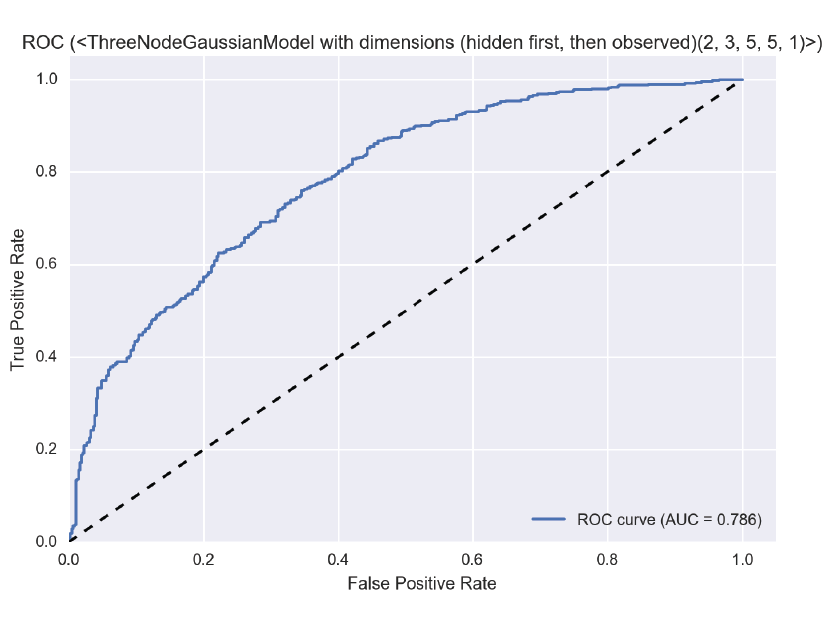
\includegraphics[width=.9\textwidth]{/Users/ijoseph/Documents/Work/Graduate-Thesis/TeX/figures/ch4_1_a.png}
  %       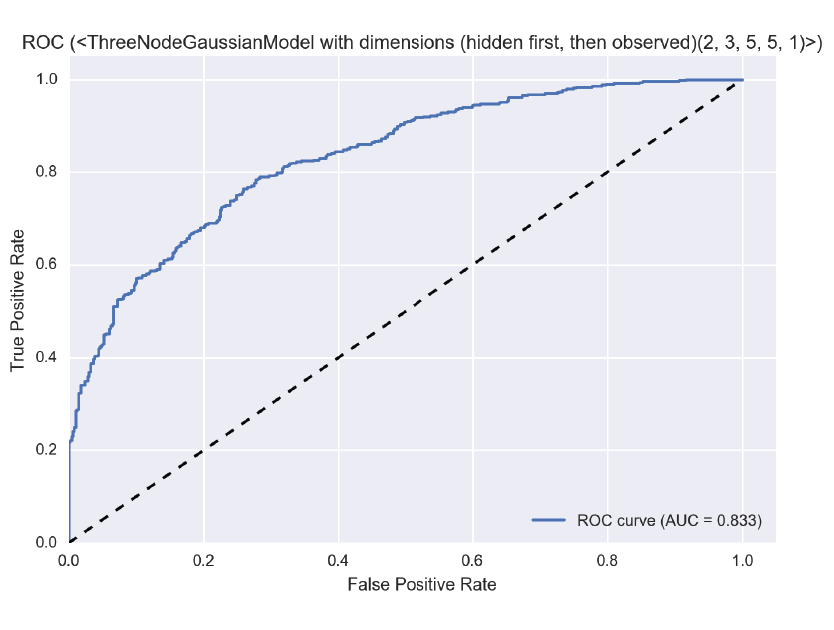
\includegraphics[width=.9\textwidth]{/Users/ijoseph/Documents/Work/Graduate-Thesis/TeX/figures/ch4_1_b.png}

  %       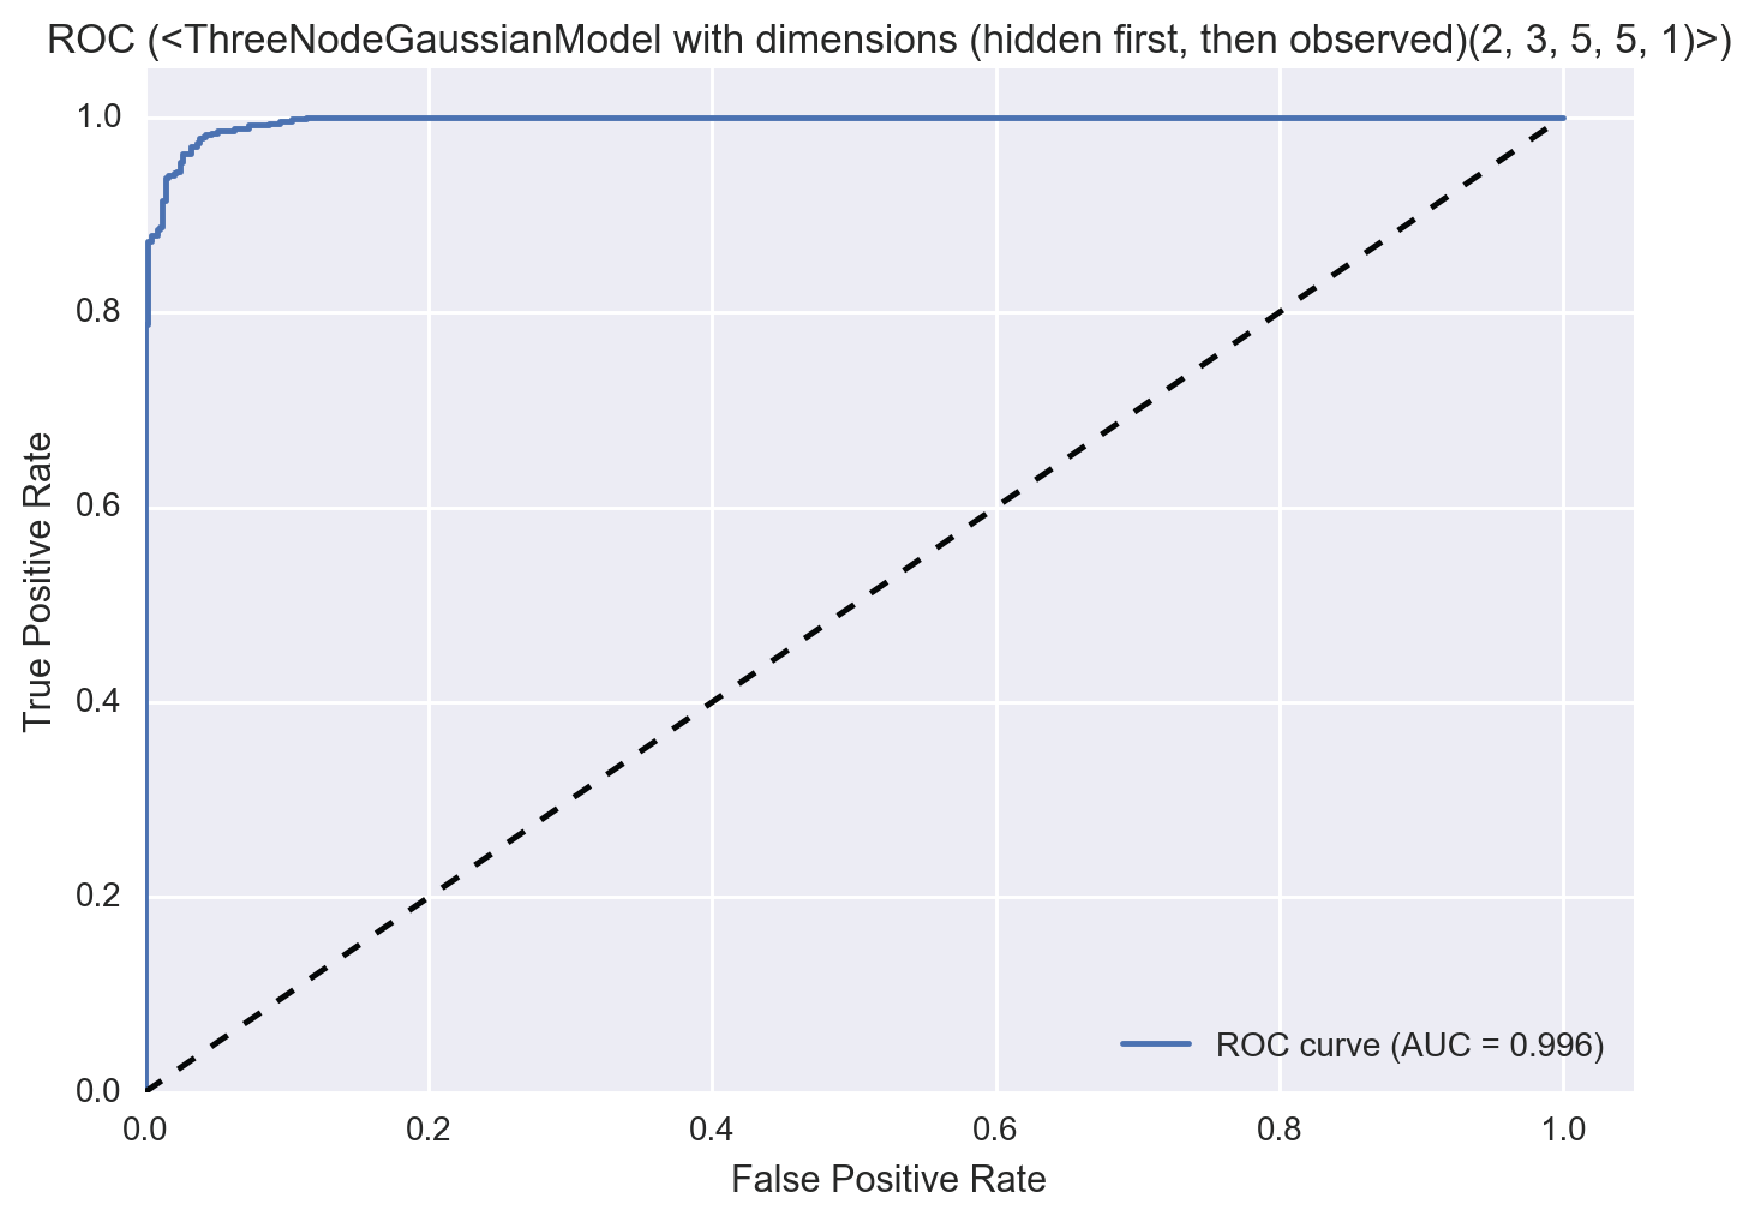
\includegraphics[width=.9\textwidth]{/Users/ijoseph/Documents/Work/Graduate-Thesis/TeX/figures/ch4_1_c.png}       
        
  %       \caption{HFAM AUC values for $e = 1$ (top) , $1.25$ (middle),
  %         $10$ (bottom)}}
  %   \end{figure}
  % \end{center}


  
  \item[$\mathbf{N=30,p=10}$] This number of samples roughly
    corresponds to that which is available from the Costello
    Lab. Here, we see a greater advantage of the model in terms of
    AUC, especially at relatively low effect-sizes. \todo{figure}
  \end{description}

\subsubsection{$\mathbf{p \gg N}$}

Secondly, we sought to assess the model's performance for data with dimensions that approximated the dimensions of real genomic data.

\begin{description}
\item[$\mathbf{N = 1\,000, p = 50\,000}$] 

First, we assessed its performance on $p = 50\,000$, which is similar to two datatypes' dimensions from the Cancer Genome Project.

Here, we found the model slightly superior than logistic regression, and requisite $e$ to be $1.25$ for what we consider adequate prediction accuracy (AUC $\appox 0.85$). 

\todo{insert figures}
\item[$\mathbf{N = 30, p = 500\,000}$] 
Secondly, we attempted to assess the model performance on  $N = 30$, $p = 500\,000$, which is similar to Costello's data size, but found performance prohibitive without further algorithmic optimization. In lieu of this, we opted to preemptively reduce dimensionality for the Costello dataset (see below).
\end{description}

\subsection{Cancer Genome Project}

First, we assessed the efficacy of the model using both expression and mutation information.

Expression information was used in the form of $z-scores$, derived as described earlier. Mutation information was used on a genic level, where any mutation occurring anywhere within a gene body resulted in a binary $1$ for that gene in that sample.

As this was the gene level, there were roughly $26\,000$ features per mutation type.

Missing information for a gene was imputed based on average for that gene across all samples for which information for that gene was present. 

Logistic regression performed poorly on this dataset, achieving an AUC of $0.5$, which was indistinguishable from chance.

HFAM performed \todo{so how'd it do after I fixed the issues.}



\subsection{Glioma prediction}

Here, we used sequencing data collected post-second surgery to see if we could assess hypermutation as having already occurred (versus prediction of future hypermutation), as preliminary attempts to predict outcome from first-surgery tissue were unpromising.

We chose to use methylation and mutation information, as these datatypes were available for the highest number of samples.

We chose the $50\,000$ most variable methylation probes, pursuant to suggestions from Dr. Matthew Grimmer as to the most cogent way to reduce methylation dimensionality. In particular, this was deemed superior to binning based on specific regions, as related glioma methylation changes often occur on a single-point basis, rather than on a large scale basis.

\todo{so how did this turn out}.


\section{Discussion}

This approach shows promise; we feel that further refinement of the approach could yield to more accurate prediction than what is shown above. In particular, we would like to implement a model tuning phase above in order to assess dimensions; we would like to use the model to integrate more than two feature types -- a relatively simple addition on what is currently implemented. We would like to use different distributions for our observed datatypes that work more cogently with mutation information -- chiefly, the multinomial distribution.

We would like to assess the model versus existing non-probabilistic methods for heterogeneous, regularized supervised prediction as well, such as collaborative regression. 
